\documentclass{report}

% The ams packages are required to insert any mathematical symbols that you may require
\usepackage{amsfonts}
\usepackage{amssymb}
\usepackage{amsmath}
\usepackage{amsthm}
% This package is used for embedding things like PDFs and JPEGs into your document
\usepackage{graphicx}
% This package is used for drawing pictures (such as trees)
\usepackage{tikz}
\usetikzlibrary{arrows,automata}
% These packages are used for adding pseudo-code to your document
\usepackage{algorithm2e}
\usepackage{algorithmic}
% This package is for if you require an appendix
\usepackage{appendix}

\usepackage{datetime}
\usepackage{fancyhdr}
\usepackage{semantic}
\usepackage[noload]{qtree}
\usepackage{comment}
\usepackage{pdflscape}
\usepackage{graphicx}
\usepackage[margin=1in]{geometry}
\usepackage{moreverb}
\usepackage{caption}
\usepackage{url}
\usepackage{layout}
\usepackage{subfig}
\usepackage{lineno}
\usepackage{bm}

\usepackage[annatar]{tengwarscript}

\newcommand{\arr}{\mathbb{R}}
\newcommand{\st}{\;\; st \;\;}
\newcommand{\nat}{\mathbb{N}}
\newcommand{\pr}{\mathbb{P}}
\newcommand{\vol}{\mbox{vol}}
\newcommand{\tengm}{\mbox{\Tmalta}}
%\newcommand{\tengm}{m}


\newtheorem{proposition}{Proposition}

\begin{document}

%\begin{titlepage}

\centering{\textsc{\huge{On the Properties of Monte Carlo Estimation of the Volume of a Convex Polytope}}}\\[1.5cm]

\centering{\textsc{\large{A Summer Project Funded by the University of Bristol's Prize Studentship Scheme}}}\\[1.5cm]

\begin{minipage}{0.4\textwidth}
\begin{flushleft} \large
\emph{Author:}\\
Tim Jones
\end{flushleft}
\end{minipage}
\begin{minipage}{0.4\textwidth}
\begin{flushright} \large
\emph{Supervisor:} \\
Dr. Rapha\"{e}l Clifford
\end{flushright}
\end{minipage}\\[1.5cm]

\vfill

\begin{abstract}
We evaluate a practical implementation of an efficient convex volume estimation algorithm, and tune its parameters such that they produce accurate results, with fewer computational steps than those deemed necessary in the theoretical papers. We find that $2^5$ steps of a hit and run random walk is sufficient to produce adequately random points and $2^{13}$ random points is enough to provide reasonable quality estimates of volume ratios. We then conclude by showing that for a convex polytope in 10 or more dimensions with 25 or more vertices, it is more efficient to use a randomised algorithm than to compute the volume exactly.
\end{abstract}

\vfill

Rendered on \today

\end{titlepage}

\clearpage

\newpage

\tableofcontents

\chapter{Introduction}

\section{Motivation and Goals}

The estimation of the volume of a convex shape in $n$ dimensions, $K$ is a long standing problem. Exactly calculating the volume of an arbitrary convex polytope is known to be \#P-complete, %cite
 but it has been shown by many authors %cite
that arbitrarily good estimates can be acquired by testing whether a polynomially bounded number of points fall within the shape. The order of this polynomial has been chipped away incrementally over many years until the most recent papers %cite simulated annealing and random walks
have successfully bounded the number of oracle queries to be within $O^*(n^4)$ and $O^*(n^5)$ respectively, stating that this brings the methods within the realms of a parctical implementation.

In this study, we will test the various features of the $O^*(n^5)$ volume algorithm by implementing a version of it in ANSI C, using the theoretical bounds as a guide to estimate good values for relevant parameters, and finally compare its overall execution time to various exact methods of volume conmputation over various simplices. We will find that the theoretical upper bounds on most parameters are very loose indeed, and that in practice far smaller values are sufficient, resulting in significant savings on real-world execution time, however the assumption of a unit-time oracle proves impractical, and when more detailed information about the shape is available, an exact method is still usually faster, despite its exponential complexity.

\section{Preliminaries}
\subsection{Notation}



\subsection{Shapes}

We will call any continuous subset of $\arr^{n}$ a shape. A convex shape, $K$, is one which satisfies

$$
\forall u, v \in K, \lambda \in [0,1] \quad (\lambda u + (1-\lambda) v) \in K
$$

Such a combination of points is known as a convex combination. More intuitively, we say that $K$ is convex if any straight line segment between any two points in $K$ lies entirely within $K$. $K$'s boundary does not ``bow inwards".

We will denote by $B$ the unit ball, that is $B = \{x \in \arr^n \st ||x|| \leqslant 1\}$, and abuse notation slightly by donoting the ball of radius $R$ by $RB$. The ball of radius $RB$ is trivially the largest convex shape that will fit within the ball of radius $RB$.

The convex hull of a set of points, denoted $h(P)$, is the set of points defined thus

$$
x \in h(P) \iff \exists u_1, u_2,...,u_k \in P, \lambda_1, \lambda_2, ..., \lambda_k  \in [0,1] \st x = \sum^{k}_{i=1} \lambda_i u_i \wedge \sum^{k}_{i=1} \lambda_i = 1
$$

Less formally, the convex hull of a set of points is the result of wrapping an elastic band around them and letting it snap tightly around them. All convex hulls are convex.

We will define the n-dimensional ice cream of radius $R$, $RI$ as the convex hull of $B$ and the point $(R,0,0,...0)$. Figure \ref{fig_ice_cream} should make the logic behind this name reasonably clear. The n-dimensional ice cream is important for this study because it is the smallest possible convex shape which contains $B$ and is tightly contained within $RB$. It will represent a pathological case for several algorithms, however as the disjoint union of a capless ball and a n-dimensional cone, its volume, whilst non-trivial, is calculable. The details can be found in Appendix \ref{app_ice_cream}.

$$
vol(RI) = %Volume of ice cream goes here - cite http://docsdrive.com/pdfs/ansinet/ajms/2011/66-70.pdf
$$

\subsection{Markov Chains and Random Walks}

A Markov Chain is a triple, $(S,P,\bm{\delta})$, where $S$ is referred to as the state space, $P = (p_{st})_{s,t \in S}$ is the transition matrix and $\bm{\delta} = (\delta_s)_{s \in S}$ is the initial probability vector. A realisation of a Markov Chain is a sequence of states, $(x_i)_{i \in \nat}$ such that $\pr (x_0 = s)=\delta_s$, and $\pr(x_i = s_i | x_0 = s_0, ..., x_{i-1} = s_{i-1}) = \pr (x_i = s_i | x_{i-1} = s_{i-1})= p_{s_{i-1}s_{i}}$. We say that $\bm{\pi}$ is a stationary distribution of the Markov Chain if, given that $\bm{\delta} = \bm{\pi}$, the marginal probabilities $\pr(x_i = t) = \pi_t$ for all $i$ and $t$.  It is a standard result from probability theory that, if one can find a probability distribution $\bm{\pi}$ such that

$$
\forall s,t \in S, \quad \pi_s p_{st} = \pi_t p_{ts}
$$

Then $\bm{\pi}$ is the stationary distribution for the chain. It should be reasonably obvious that, if $p_{ij} = p_{ji}$ for all pairs of states, then $\bm{\pi}$ is a constant. If a stationary distribution exists for a chain, then, regardless of $\bm{\delta}$, $lim_{i-> \infty} \pr {x_i = s} = \pi_s$.

A random walk through a shape is a markov chain whose state space approximates the interior of a shape. We will use a random walk to sample uniformly at random from the inerior of a shape. By selecting a walk that satisfies $p_{ij} = p_{ji}$, we can can trace some number of steps from this walk, and return the state after some number of steps. The walk we use will be the Hit and Run Walk %cite Fast and Fun
which has been shown both theoretically and in practice to rapidly approach its stationary distribution, requiring a very small number of steps to produce good randomness. For a walk in the interior of $K$, starting at $\bm{x}_0$, the Hit and Run walk selects a line uniformly at random passing through $\bm{x}_0$ and contained entirely within $K$, then moves to a point uniformly distributed along this line. We will aim to see how many times this must be repeated before the resulting point is uniformly distributed within $K$.

\subsection{The Volume Estimation Algorithm}

The algorithm we will use follows %lovasz paper
with three differences. Rather than generating random points using the ball walk, we generate points with Hit and Run, which experimental results show mixes significantly faster than the ball walk. Rather than using $2$ as the base for our exponents, we use $e$. At each stage, if the estimated volume is higher than it is possible for the volume to actually be, we will clamp the estimated volume back down to its maximum.

To estimate the volume of some shape, $K$, we choose a sequence of shapes, $K_0 \subseteq K_1 \subseteq ... \subseteq K_p$, such that the volume of $K_0$ can be computed easily, $K_p = K$, and we can estimate the ratios $\frac{vol(K_{i+1})}{vol(K_i)}$ easily. For our algorithm, we will chose the shapes $K_i = (e^{i/n}B) \cap K$ for $i = 0, ..., n \log (R)$. Since $B \subseteq K \subseteq RB$, this satisfies our first two conditions. We can then estimate the ratios by sampling uniformly at random from $K_i$ and counting the number of points which fall into $K_{i-1}$. Modifying an oracle that samples from $K$ such that it samples from $K_i$ is fairly easy, and ratio of volumes can be estimated as the fraction of uniformly generated random points in $K_i$ that fall into $K_{i-1}$.

\chapter{Experiments}

\section{Mixing time}\label{sec_mix}

Our first experiment will attempt to bound the mixing time of the Hit and Run random walk in a convex shape. The hit and run walk is known to mix rapidly \cite{Lovasz98, Lovasz05} in the sense that the number of steps needed for the walk to reach a uniform ditribution is $O^{*}(n^2)$, however this result actually shows that the walk can only be guaranteed to mix after over $10^{10} n^2$ steps. Performing $10^{10} n^2$ steps in a hit and run walk will take a very long time indeed, so if possible we would like to use far fewer.

We will generate 1,000 points with a hit and run walk using a variable number of steps, and perform a statistical test against a known uniform distribution to see if the walk has mixed properly. For each set of points generated by each method, we will compute the distance from the point to its nearest neighbor, then compare the distribution of distances by the Kolmogorov-Smirnov test. If the test passes at the 5\% level, then we will judge the walk to be well-mixed.

It is not clear which shape is likely to constitute a pathological case for the hit and run walk; the ice cream has the smallest volume, and so in a sense fewer points need to be chosen from, but also has the tighest possible corner, in which the walk is most likely to get stuck. By contrast, the ball has the largest volume and no corners. We will test both shapes. Uniformly distributed random points can be generated from a ball fairly easily, and uniform random points can be generated from an ice cream by simple rejection sampling. To keep our search reasonably short, we will restrict ourselves to only testing numbers of steps equal to natural powers of 2. Due to the extreme scaling of rejection sampling from an ice cream, it is not feasible to test any more than 8 dimensions on a home computer; though the wall clock times are not one of the variables we will be analysing, this information was still gathered for this experiment. If it took $t$ seconds to rejection sample 1,000 points from $n$ dimensions, then it took roughly $10t+t$ to sample the same number of points from $n+1$ dimensions.

We conclude from these tests that, for up to 8 dimensions, using $2^5$ steps produces adequately random points. Whilst there was one exception to this, namely the number of steps to sample from an ice cream where $n=3$, it is also true that a very large number of tests was performed, so it's likely that this one exception is just a statistical outlier. Given the difficulty of taking a hit and run step, this is still a relatively expensive random number generator, but nowhere near the theoretical upper bound of $10^{10}$. This is relieving, and we will use these 32 steps in the random walk for the following experiments.

Running gprof over the code as it executes reveals that roughly 60\% of the time for each random walk is spent executing the binary search to find the boundaries of the convex shape, and even a simple oracle such as one for the ball $RB$ consumes another 20\% of the walk time. If further work is to be performed on the algorithm, authors may be well advised try and control this time.

\section{Threads per stage}\label{sec_error}

We will now see how the number of threads per phase influences the accuracy of an estimate. In the paper describing our particular estimation method, it is stated that, for an n-dimensional shape, in order to achieve an error of $\varepsilon$, we should use $400\frac{n\log n}{\varepsilon^2}$ threads per stage. This, again, is an upper bound, and we would like to show that it is loose. We shall vary the number of threads used per stage, and see how the distribution of estimates varies with this value. As before, we will use both the ice cream and the ball to respectively maximise and minimise the ratios between successive shapes. Our analysis here will be largely visual, since any returned value from this algorithm might be considered valid for a sufficiently large value of epsilon.

In all cases the errors decrease fairly rapidly, with estimates being easier to acquire for the ball than for the ice cream. The ice cream is very much the pathological case here. These figures can be used to read off the minimum number of threads needed to get an estimate of a given quality, but it is interesting to note that estimates show a clear tendency to converge towards slightly incorrect values. It is possible that this convergence is due to numerical instability. Note that an inverse polynomial relationship with $\varepsilon$ remains apparent in the graph of greatest absolute error.

We also depict the greatest errors made on each shape in terms of apsolute error. Because of the vast number of graphs, figure \ref{fig_histograms} will only show a few.

\begin{figure}
\centering
\subfloat[Histograms for the ball estimates]{
	\includegraphics[width = 0.4 \textwidth]{./images/6-dimensions_ball_3d.png}
}
\subfloat[Histograms for the ice cream estimates]{
	\includegraphics[width = 0.4 \textwidth]{./images/6-dimensions_ice_cream_3d.png}
} 
\\

\subfloat[The worst mistakes made in the ball estimates]{
	\label{fig_2d_ball}
	\includegraphics[width = 0.4 \textwidth]{./images/6-dimensions_ball_2d.pdf}
}
\subfloat[The worst mistakes made in the ice cream estimates]{
	\includegraphics[width = 0.4 \textwidth]{./images/6-dimensions_ice_cream_2d.pdf}
	\label{fig_2d_ice_cream}
}
\caption{Variance in errors for various shapes, measured in different ways}
\label{fig_histograms}
\end{figure}

%Plot minimum number of threads needed for greatest absolute error to drop below 0.2?

So, reading off from figures \ref{fig_2d_ice_cream} and \ref{fig_2d_ball}, in a 6-dimensional ice cream our estimates all become correct for $\varepsilon > 0.1$ for any number of threads greater than $2^11 = 2,048$. For a 6-dimensional ball to within an error of $0.1$, we need more like $2^{13} = 8,192$. In all cases, the error drops below $0.2$ for $2^{13}$ threads per stage. The papers suggest that at least $400\frac{n\log n}{\varepsilon^2} \approxeq 620,000$ threads are necessary for each stage. Once again, the upper bound is very loose indeed.

\section{Computation Time for Convex Shapes}\label{sec_time}

It's now time to test the practicalities of this algorithm on a series of convex shape, against already established methods of exact volume computation. The code used for comparison is the same as that used in \cite{Bueler98}
and was run over a series of randomly generated convex shapes. Each shape is the convex hull of the box $[-1,1]^n$, and some variable number of points on the ball of radius $\sqrt n$. We will randomly generate series of shapes in each dimension, increasing the number of points on the hull, and seeing how this affects the time for a volume estimation to complete using the values found above by experimentation

All experiments were conducted on the same hardware and in the same operating system, using the same time metric. The processor is an Intel i5-2500k in a Gigabyte Z68AP-D3 motherboard, connected to 8 GiB of 1,600 MHz dual-channel DDR3 RAM. The programs were both compiled onto a 64-bit install of Ubuntu 12.04 virtualised by Oracle VM Virtualbox with access to 2GiB of RAM. Each time is measured in elapsed clock cycles divided by the number of clocks per second. Using this processor time removes the possibility of error due to other running processes The actual wall-clock time is significantly longer, but the listed times ignore the time spent by the OS performing other processes, as well as the overhead incurred for virtualisation. Neither program is designed to exploit any more than a single processor core, since this would require extensive modification of the code from \cite{Bueler98}.

Initially, the oracle was implemented with a linear programming solver. A point ${\bm p}$ lies within the convex hull of a set of $v$ vertices $\{{\bm x}^1, {\bm x}^2, {\bm x}^3, ..., {\bm x}^v\}$ iff there exists a vector ${\bm \lambda}$ such that

\begin{align*}
\lambda_1 x^1_1 + \lambda_2 x^2_1 + ... + \lambda_k x^v_1 &= p_1 \\
\lambda_1 x^1_2 + \lambda_2 x^2_2 + ... + \lambda_k x^v_2 &= p_2 \\
&\vdots \\
\lambda_1 x^1_n + \lambda_2 x^2_n + ... + \lambda_k x^v_2 &= p_n \\
\lambda_1 + \lambda_2 + ... + \lambda_v &= 1
\end{align*}

This defines the feasible region of an LP problem, which an LP solver can then inspect to see if any solutions for ${\bm \lambda}$ exist. The solver used was Gurobi, chosen simply because it is the fastest availalbe LP solver. Whilst the LP solver is fast, it will be given vast numbers of LPs to solve, leading to some slow execution times.

This particular method of representing a polytope is known as vertex representation, or v-representation. It is also possible to represent a polytope as two sets of halfspaces. A point lies in a convex polytope iff it is below some set of halfspaces and above some other set of halfspaces. Each halfspace forms one facet of the polytope. Representing a polytop as a set of halfspaces is known as the h-representation. The fastest exact methods require the shape to be converted from v-representation to h-representation before the volume can be computed. Facet enumeration, the problem of performing this computation, is solvable in $O(vl(v,n)f)$ time\cite{Fukuda97}, where $f$ is the eventual number of facets, and $l(v,n)$ is the complexity of solving a linear programming problem in $n$ variables and $v$ constraints. LP solving is exponential in its worst case\cite{Klee72}, but is known to be efficient when used against real-world problems. It is also known that when the vertices are generated in this way, on average $f \in \Theta(v)$. In practice, however, I have found facet enumeration to be very slow - slower in fact than estimating a polytope's volume.

Generating a large sample size across several dimensions and several shapes would be very difficult. Where previously we could comfortably generate thousands of data points, here we will have to restrict ourselves to 5 samples from each experiment. In each experiment, we will start with the $n$-dimensional cross-polytope $\{{\bm x} | \sum^n_{i=1}|x_i| \leqslant R\}$, add either 0, 25, 50, 75 or 100 extra vertices, uniformly distributed over the surface of the ball of radius $R$, then estimate the volume of their convex hull. From the definition of the cross-polytope, it is fairly easy to show that it is exactly the convex hull of the points $\pm R{\bm e}_i$ for $i \in \{1,2,...,n\}$, where ${\bm e}_i$ is the vector whose $i^{th}$ component is 1, and all others are 0, so each cross-polytope adds exactly $2n$ vertices to the v-representation. Since $R=\sqrt{n}$, this cross-polytope always contains the unit ball, see Appendix \ref{app_cross_polytope} for details. These initial points are necessary, since the probability of containing the entire unit ball is low, and there is no easy way to check whether the unit ball is even contained by the random shape, cf Appendix \ref{app_balls}.

The data will then be passed into an exact solver, which will attempt to convert the shape from its v-representation to an h-representation, then compute the exact volume via the Hybrid Orthomormalisation Technique \cite{Bueler98}. If any stage takes longer than one hour of processor time, it will be terminated early. The number of the experiment will be used as a random number seed; the Mersenne Twister will be seeded from 1, 2, 3, 4, and 5, depending on the experiment, and the Ziggurat will be seeded from a number generated by the Mersenne Twister. Anything that remains unclear can hopefully be explained by reading the code. %cite code


\begin{table}[h]
\centering
\begin{tabular}{| c || p{1cm} | p{1cm} | p{1cm} | p{1cm} | p{1cm}|}
\hline
&\multicolumn{5}{p{6cm}|}{Average Computation Time for $v$ Extra Points (minutes)} \\
\hline
Number of Dimensions & $v = 0$ & 25 & 50 & 75 & 100\\
\hline
4  & 3.88  & 4.85  & 5.53  & 6.16  & 6.79  \\
5  & 6.64  & 9.40  & 10.81 & 12.20 & 13.51 \\
6  & 8.51  & 13.02 & 14.62 & 16.49 & 18.38 \\
7  & 10.05 & 16.77 & 18.63 & 20.83 & 23.84 \\
8  & 12.58 & 19.93 & 24.86 & 27.32 & 36.29 \\
9  & 12.94 & 23.91 & 29.39 & 37.76 & 41.38 \\
10 & 16.29 & 28.31 & 36.93 & 43.20 & 53.53 \\
\hline
\end{tabular}
\caption{Average Computation Times for Volume Estimation}
\label{tab_estimation_time}
\end{table}


\begin{table}[h]
\centering
\begin{tabular}{| c || p{1cm} | p{1cm} | p{1cm} | p{1cm} | p{1cm}|}
\hline
&\multicolumn{5}{p{6cm}|}{Average Conversion Time for $v$ Extra Points (seconds)} \\
\hline
Number of Dimensions & $v = 0$ & 25 & 50 & 75 & 100\\
\hline
4 & 0.0 & 0.0   & 0.0    & 0.0    & 0.0 \\
5 & 0.0 & 0.0   & 0.0    & 0.2    & 0.2 \\
6 & 0.0 & 0.2   & 0.4    & 1.0    & 2.6 \\
7 & 0.0 & 0.0   & 1.0    & 5.4    & 14.8 \\
8 & 0.0 & 2.0   & 40.4   & 268.0  & 652.0 \\
9 & 0.0 & 9.0   & 360.2  & 2292.0 & $\bot$ \\
10& 0.0 & 353.4 & $\bot$ & $\bot$ & $\bot$ \\
\hline
\end{tabular}
\caption{Average Times to convert from v-representation to h-representation. Times of $\bot$ denote a conversion which was timed out for taking more than an hour.}
\label{tab_conversion_time}
\end{table}

Table \ref{tab_estimation_time} shows fairly unsurprising linear scaling across both axes. Table \ref{tab_conversion_time} suggests that the conversion from v-representation to h-representation is exponential in both directions. This isn't entirely unexpected - we already know that the shape will always have an exponential number of facets with respect to $n$, and for shapes more complex than 50 points in 10-dimensional space the time to convert from v to h representation is significantly longer than the time to simply estimate the shape's volume via the monte-carlo techniques. Indeed, in one of the preliminary experiments, a shape with $n=10$ and $v=100$ was input into the conversion code for an evening. After 6 hours, the output reported that it had completed $75\%$ of its iterations. Each iteration appeared to take longer than the previous one, but the code will have needed at least 8 hours in total to complete the conversion. Compare this to the 53 minutes needed to estimate one of these volumes to within a reasonable degree of accuracy.

After the conversion, the times to compute volumes are barely worth reporting. The longest time across all shapes was achieved for $n=9$ and $v = 75$, taking 274.9 seconds - negligible in comparison to the $2292.0$ seconds taken for conversion, a trend which continued for all the generated shapes.

\section{Conclusions and Future Work}

Given a vertex representation for a convex shape in $n$ dimensions, using exact methods to compute its volume remains a viable option for $n<9$ and a reasonably simple shape, however as the number of dimensions grows beyond this, it becomes highly impractical to continue with exact methods, and monte-carlo based volume estimation becomes a very attractive option indeed. The specific parameters needed for these operations are generally significantly lower than those theorised, meaning that significant savings can be made for a practical implementation.

However, a convex shape in $10$ dimensions with $120$ vertices is still fairly simple, yet requires roughly an hour of processor time to process. Even estimating the volume of a convex shape is very difficult, and these methods do not provide a substitute for domain specific knowledge and careful consideration of the shapes at hand.

Some questions remain unanswered by this study. These shapes were deliberately chosen to fulfil the properties required by the volume estimation algorithms, however any shape can be transformed to fulfil these properties by sampling a large number of points uniformly, then transforming these such that they contain the unit ball and are contained within a ball of fixed radius. These methods were simply untested in this study, but there are probably also useful experimental results on the number of points necessary to transform a shape ``well". With more computational power, more data points could be generated leading to more information on how these methods scale into more dimensions - a supercomputer cluster could easily generate data for shapes in several hundred dimensions, but these data had to be gathered from a single home computer. It would also be interesting to see how well these methods could be parallelised - each random walk can certainly be simulated independently of all others, so it would probably be possible to scale these methods up to some very large clusters.

To finish, the appendices will investigate various subsidiary features of these methods.

\appendix
\chapter{The Ice Cream} \label{app_ice_cream}

The $n$-dimensional ice cream of radius $R>1$, denoted $RI$ is the convex hull of the unit ball and the point $(R,0,0...,0)$. In this section, we will simply argue that its volume is

$$
\vol_n(RI) = \frac{R-h}{n} \vol_{n-1}(rB) + \vol_n(B) - \left(\frac{1}{2}\vol_n(rB) I_{\frac{2rh-h^2}{r^2}}\left(\frac{n+1}{2}, \frac{1}{2}\right)\right)
$$

With $h = \frac{1}{R}$, $r = \sqrt{1-\frac{1}{R^2}}$ and $I_x(a,b)$ is the incomplete beta function, defined thus:

$$
I_x(a,b) = \frac{\int^x_0 t^{a-1}(1-t)^{b-1}dt}{\int^1_0 t^{a-1}(1-t)^{b-1} dt}
$$

We will show that the shape can be written as the union of two disjoint sets. Let
$$
S = B \cap \left\{\bm{x} \in \arr^n | x_1 \leqslant \frac{1}{R}\right\}
$$
And
$$
W = \left\{\bm{x} + \left(\frac{1}{R}, 0, ..., 0\right) | x_1 > 0 \; \wedge \; \sum^{n}_{i=2} x_i^2 < \left(\frac{\sqrt{1-R^{-2}}}{R-R^{-1}} x_1\right)^2 \right\}
$$

We will call $S$ the scoop, and is the spherical part of the ice cream near the origin, and $W$ the wafer, the conical part nearer to the point $(R,...,0)$. These two shapes are clearly disjoint, so the volume of the ice cream is the sum of the volumes of the scoop and the wafer. We will show that these shapes partition the ice cream by showing that any line tangent to the unit ball through $(R,0,...,0)$ touches the ball at a point whose first coordinate is $\frac{1}{R}$.  The set of points touching the surface of an $n$-ball whose first coordinate is $\frac{1}{R}$ is an $(n-1)$-ball of radius $\sqrt{1-R^{-2}}$, and the distance from this surface to $(R,0,...,0)$ is $1-\frac{1}{R}$. The convex hull of points on an $n-1$ dimensional surface with a point normal to the surface is an $n$-dimensional hypercone. This hypercone is the wafer, the remainder is the scoop. Most of this will manifest as simple but non-obvious geometry, so it is worth describing fully.

\begin{proposition}
A line tangent to the unit $n$-ball that passes through $(R,0,...,0)$ intersects the surface of the $n$-ball at a point whose first coordinate is $\frac{1}{R}$ at a distance $\sqrt{1-\frac{1}{R^2}}$ from the line from the origin to $(R,0,...,0)$
\end{proposition}

The situation is as depicted in figure \ref{fig_ice_cream_annotated}. $O$ is the origin, $B$ is the point $(R,0,...,0)$, and $A$ is any point on the surface of the unit $n$-ball such that $AB$ is tangent to the surface. $OAB$ is a right angle. $C$ is the point such that $O$, $C$ and $B$ are colinear, and $ACB$ is a right angle. Since $OAB$ is a right angled triangle, $|AB| = \sqrt{R^2-1}$. From the law of sines, $\sin(AOB) = \frac{\sqrt{R^2-1}}{R}$, so $\cos(AOB) = \frac{1}{R}$, so $|OC| = \frac{1}{R} = h$, and $|AC| = \sqrt{1-\frac{1}{R^2}} = r$, as required.

We also have that $|CB| = R-h$, and that the points on the surface of the unit ball whose first coordinate is $h$ is an $(n-1)$-ball of radius $r$. This tells us that the wafer is an $n$-dimensional hypercone of height $R-h$ and whose base is the $(n-1)$-ball of radius $r$.

\begin{figure}
\centering
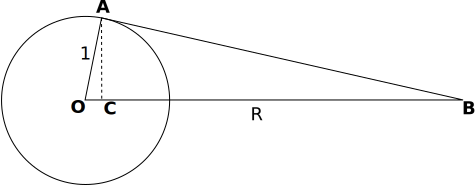
\includegraphics{./images/ice_cream_annotated.pdf}
\caption{Annotated components of an ice-cream, projected onto the 2-d plane. Points are in bold font, and variables in italic.}
\label{fig_ice_cream_annotated}
\end{figure}

\begin{proposition} \label{prop_vol_wafer}
The volume of the wafer is $\frac{R-h}{n} \vol_{n-1}(rB)$
\end{proposition}

The set of points in the wafer at a distance of $t$ from point $B$ is exactly the set of points in the $(n-1)$-ball of radius $\frac{rt}{R-h}$, so

\begin{align*}
\vol(W)
&= \int^{R-h}_{0} \vol_{n-1}\left(\frac{t}{R-h}rB\right) dt \\
&= \frac{1}{R-h}^{n-1} \vol_{n-1}(rB) \int^{R-h}_0 t^{n-1}dt \\
&= \frac{R-h}{n} \vol_{n-1}(rB)
\end{align*}
As required.

\begin{proposition} \label{prop_vol_scoop}
The volume of the scoop is $\vol_n(B) - \left(\frac{1}{2}\vol_n(rB) I_{\frac{2rh-h^2}{r^2}}\left(\frac{n+1}{2}, \frac{1}{2}\right)\right)$
\end{proposition}

The scoop is exactly a unit hypersphere without a hyperspherical dome. The volume of an $n$-spherical dome of height $h$, radius $r$ is $\frac{1}{2}\vol_n(rB) I_{\frac{2rh-h^2}{r^2}}\left(\frac{n+1}{2}, \frac{1}{2}\right)$, as proven in \cite{Li11}, so the volume of the scoop is $\vol_n(B) - \left(\frac{1}{2}\vol_n(rB) I_{\frac{2rh-h^2}{r^2}}\left(\frac{n+1}{2}, \frac{1}{2}\right)\right)$

Combining propositions \ref{prop_vol_wafer} and \ref{prop_vol_scoop}, we have the volume of the entire ice cream.

\chapter{The Cross Polytope} \label{app_cross_polytope}

In this appendix, we will show that the cross polytope, $X = \{\bm{x} | \sum^n_{i=1}|x_i| \leqslant R\}$, always contains the unit ball, $B$, for $R \geqslant \sqrt{n}$. That is, $R \geqslant \sqrt{n} => B \subseteq X$. Let $||\bm{x}||_p$ denote the $p$-norm of ${\bm x}$, defined:

$$
||\bm{x}||_p = \sqrt[p]{\sum^n_{i=1} |x_i|^p}
$$

So $X$ is the set of points satisfying $||\bm{x}||_1 \leqslant R$ and $B$ is the set of points satisfying $||\bm{x}||_2 \leqslant 1$. Let ${\bm x}, {\bm y} \in \arr^n$. The Cauchy-Schwarz inequality states that:

$$
\left(\sum^n_{i=1} x_i y_i\right)^2 \leqslant \sum^n_{i=1} x_i^2 \sum^n_{i=1} y_i^2 
$$
By choosing $y = (1,1,...,1)$, we have that for any ${\bm x} \in \arr^n$
$$
\left(\sum^n_{i=1} |x_i| \right)^2 \leqslant n \sum^n_{i=1} |x_i|^2
$$
Taking square roots of both sides, we have that $||\bm{x}||_1 \leqslant \sqrt{n} ||\bm{x} ||_2$. Now, ${\bm x} \in B$ iff $||{\bm x}||_2 \leqslant 1$, which implies that $||{\bm x}||_1 \leqslant \sqrt{n}$, so ${\bm x} \in X$. $x \in X => x \in B$, as required.


\end{document}